\documentclass[10pt]{article}
\usepackage[french]{babel}
\usepackage[utf8]{inputenc}
\usepackage[T1]{fontenc}
\usepackage{amsmath}
\usepackage{amsfonts}
\usepackage{amssymb}
\usepackage[version=4]{mhchem}
\usepackage{stmaryrd}
\usepackage{graphicx}
\usepackage[export]{adjustbox}
\graphicspath{ {./images/} }
\usepackage{caption}

\begin{document}
\captionsetup{singlelinecheck=false}
\section*{Exercice n ${ }^{\circ} 1$ : Question de cours : 2 pts}
On considère un avion dans sa phase d'atterrissage, il passe d'une altitude $A$ à une altitude $B$. On notera $\mathrm{z}_{\mathrm{A}}$ et $\mathrm{z}_{\mathrm{B}}$ les altitudes des deux points.

\begin{enumerate}
  \item Faites un schéma présentant la situation en y faisant apparaître Le poids de l'avion au point A et au point B .
  \item Démontrer la formule $\mathrm{W}_{\mathrm{AB}}(\vec{P})=\mathrm{P}\left(\mathrm{z}_{\mathrm{A}}-\mathrm{z}_{\mathrm{B}}\right)$.
\end{enumerate}

\section*{Exercice $\mathrm{n}^{\circ} 2$ : Remonte pente : 8 pts}
Un skieur gravit à la vitesse constante $\mathrm{v}=9.0 \mathrm{~km} / \mathrm{h}$ une portion $\mathrm{AB}(\mathrm{AB}=150 \mathrm{~m})$ de piste rectiligne, inclinée d'un angle $\alpha=35^{\circ}$ par rapport à l'horizontale.

Il est tractée par la pêche d'un remonte pente qui exerce sur le skieur une force constante $\vec{F}$ de valeur $\mathrm{F}=590 \mathrm{~N}$, cette force étant inclinée d'un angle $\beta=25^{\circ}$ par rapport à la direction de la piste.\\
Le skieur, équipé, a une masse de 85 kg .\\
On note $\vec{P}$ le poids du skieur et de son équipement. La réaction de la piste $\vec{R}$ est décomposée en deux forces : on note $\overrightarrow{R n}$ la réaction normale de la piste et $\overrightarrow{\mathrm{f}}$ la force de frottement exercée par la piste sur le skieur.

\begin{enumerate}
  \item Le système étudié est le skieur et son équipement de ski.\\
Quel référentiel utilise t-on pour décrire le mouvement du système et pourquoi ? 0.5 pt
  \item Légender le schéma ci-contre en indiquant le nom des forces extérieures qui s'exercent sur le système. 0.5 pt
\end{enumerate}

\begin{figure}[h]
\begin{center}
  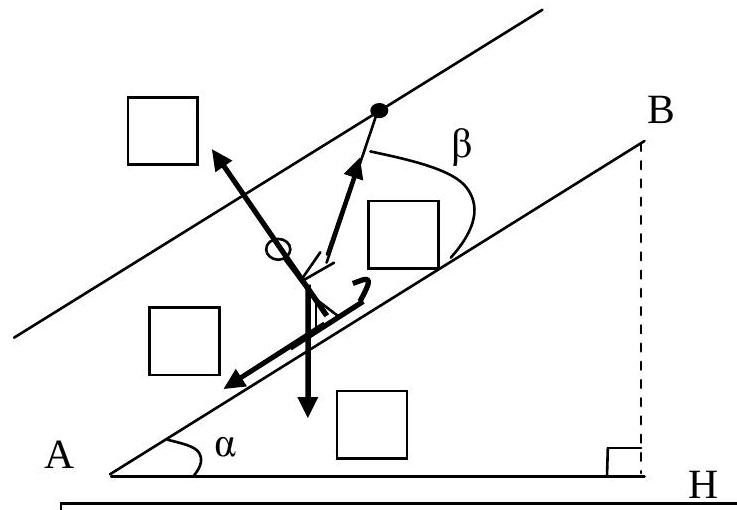
\includegraphics[alt={},max width=\textwidth]{30be3be1-ac13-4fe1-b50f-0d9387ef7d46-1_510_737_1334_1043}
\captionsetup{labelformat=empty}
\caption{Rq : Sur ce schéma, nous rappelons que $\vec{f}$ a été schématisé sans connaître son sens réel. Sa projection sur l 'axe orienté donne $+\mathbf{f}$.}
\end{center}
\end{figure}

\begin{enumerate}
  \setcounter{enumi}{2}
  \item Calculer le poids du système étudié. $(\mathrm{g}=10 \mathrm{~N} / \mathrm{kg}) \quad 0.5 p t$
  \item Calcul de la force de frottements exercée par la piste :\\
a. Le système étudié est-il pseudo-isolé ? oui/non pourquoi (deux arguments) ? 0.5 pt\\
b. Si oui, donner la relation vectorielle liant les forces extérieures appliquées au système. $0.5 p t$\\
c. Projeter cette relation sur un axe parallèle à la piste afin de déterminer la valeur de cette force de frottements. Donner également sa véritable orientation.\\
(il faudra orienter l'axe de projection et tenir compte de la remarque faites sous le schéma.). 2 pts
  \item On donne la valeur de la force de frottements exercée par la piste $\mathrm{f}=47 \mathrm{~N}$.\\
a. Calculer pour le déplacement AB , les travaux des différentes forces $(\vec{P}, \overrightarrow{R n}, \vec{f}, \vec{F})$ s'exerçant sur le système skieur + équipement. Dire si les travaux sont moteurs, résistant, ou nul. 2 pts\\
b. Calculer la puissance de la force exercée par la perche $\mathrm{P}(\vec{F}) .2$ pts
\end{enumerate}


\end{document}
